%%%%%%%%%%%%%%%%%%%%%%%%%%%%%%%%%%%%%%%%%%%%%%%%%%%%%%%%%%%%%%%%%
% Dissertacao de Mestrado / Dept Fisica, CFM, UFSC              %
% Andre@UFSC - 2011                                             %
%%%%%%%%%%%%%%%%%%%%%%%%%%%%%%%%%%%%%%%%%%%%%%%%%%%%%%%%%%%%%%%%%

%:::::::::::::::::::::::::::::::::::::::::::::::::::::::::::::::%
%                                                               %
%                          Capítulo 3                           %
%                                                               %
%:::::::::::::::::::::::::::::::::::::::::::::::::::::::::::::::%

%***************************************************************%
%                                                               %
%                         Crossmatch                            %
%                                                               %
%***************************************************************%

\chapter{Crossmatch entre \SDSS/\starlight e \galex}
\label{sec:Crossmatch}

Tradicionalmente astrônomos armazenam seus dados em arquivos texto ou binários
contendo um registro por linha, de um forma tecnicamente conhecida como {\em
flat file}. Buscas neste tipo de banco de dados são feitas examinando
individualmente cada registro do arquivo. Com o volume de dados obtido pelo
\galex (aproximadamente 222 milhões de objetos, 34 mil campos)\citneed, o uso de
arquivos simples para armazenamento de dados se torna inviável.\citneed É
preciso ``profissionalizar'' o gerenciamento de dados de um {\em survey} desta
escala.


%***************************************************************%
%                                                               %
%              Crossmatch - Banco de dados do SDSS              %
%                                                               %
%***************************************************************%

\section{Banco de dados do \SDSS}

Um dos maiores responsáveis pela promoção do uso de bancos de dados relacionais
na astronomia é o projeto {\em Sloan Digital Sky Survey} (\SDSS). Inicialmente o
\SDSS utilizou um {\em sistema de gerenciamento de banco de dados orientado a
objetos} \citep{Maier1986} (OODBMS, na sigla em inglês). Após pouco mais de um
ano a abordagem se mostrou inadequada: entre os principais problemas, uma
linguagem de {\em query} inadequada e performance ruim. O motivo, segundo
\citet{Thakar2004}, foi a incapacidade da empresa desenvolvedora do OODBMS em
prover novas funcionalidades requisitadas pelo projeto e correção de {\em bugs},
bem como em acompanhar o crescimento da performance do {\em hardware}.

\subsection{Migração de OODBMS para RDBMS}
\label{sec:CrossMatch:SDSS:MigracaoRDBMS}

Todo o banco de dados do \SDSS foi migrado para um {\em sistema de gerenciamento
de banco de dados relacional} \citep{Codd1970} (RDBMS, na sigla em inglês) num
esforço guiado por \citet{Thakar2004}. RDBMS pode ser considerado o padrão da
indústria. Praticamente todas as linguagens de programação tem bibliotecas de
interface às implementações de RDBMS comerciais mais comuns (Oracle, IBM e
Microsoft, Postgres). Há uma diversidade de ferramentas para desenvolvimento e
gerenciamento de RDBMS. E talvez o maior benefício de todos, o acesso aos dados
é feito utilizando uma linguagem padronizada: {\em Simple Query Language}, ou
simplesmente SQL \citep{Chamberlin1974}. A migração dos dados do \SDSS para um
RDBMS comercial implicou num aumento significativo da performance do acesso aos
dados, e resultou no desenvolvimento do {\em SkyServer}\footnote{\SDSS
SkyServer: \url{http://skyserver.sdss.org/}}. O servidor de banco de dados
escolhido pelo \SDSS foi o {\em Microsoft SQL Server}.

A comparação entre OODBMS e RDBMS no caso particular do \SDSS não implica
necessariamente a superioridade do segundo em relação ao primeiro. Tanto a
abordagem orientada a objetos quanto a abordagem relacional tem suas vantagens e
desvantagens. O estudo de caso do \SDSS é apenas uma evidência anedótica em
favor do uso de bancos de dados relacionais. No entanto, para aplicações
semelhantes ao \SDSS -- {\em surveys} astronômicos com volumes imensos de dados
-- vale a pena apostar no sucesso dos RDBMS.

\subsection{{\em SkyServer}}
\label{sec:CrossMatch:SDSS:SkyServer}

O {\em SkyServer} é um {\em website} (figura \ref{fig:TelaDoSkyServer}) que
provê acesso aos dados armazenados no banco de dados do \SDSS
\citep{Szalay2002}. O acesso mais simples pode ser feito através de um atlas de
locais famosos ({\em famous places}), que mostra imagens coloridas de objetos
celestes conhecidos. Há formulários para buscas mais sérias, gerando coleções de
imagens, espectros e tabelas de dados. No {\em SkyServer} é possível fazer
buscas avançadas utlizando SQL, embora haja limites de tempo de execução e de
quantidade de objetos retornados. Esta limitação é contornada através do sistema
{\em CasJobs}, que é tratado na seção \ref{sec:CrossMatch:SDSS:CasJobs}.

É importante ressaltar que é possível (de fato, a equipe do \SDSS encoraja)
criar {\em mirrors}\footnote{{\em Mirror}: Espelho, em inglês. Clone de um {\em
website}.} do {\em SkyServer}. Tanto o banco de dados do \SDSS quanto o código
fonte do {\em SkyServer} estão disponível no próprio {\em website} do {\em
SkyServer}. Há um clone do banco de dados do {\em Data Release} 8 do \SDSS no
servidor {\em CasJobs} do \starlight \footnote{{\em CasJobs} do \starlight:
\url{http://casjobs.starlight.ufsc.br/casjobs/}}.

\begin{figure}
	\includegraphics[width=1.0\columnwidth]{figuras/skyserver.eps}
	\caption[Telas do {\em SkyServer}.]
	{Telas do {\em SkyServer}. À esquerda, formulário para submeter uma {\em
	query} SQL. À direita, ferramenta {\em Explore} mostrando a galáxia NGC 799.}
	\label{fig:TelaDoSkyServer}
\end{figure}

\subsection{{\em CasJobs}}

\label{sec:CrossMatch:SDSS:CasJobs}
O {\em Catalog Archive Server Jobs} ({\em CasJobs}) é um serviço online
desenvolvido pela equipe do \SDSS para expandir a capacidade do {\em SkyServer}
\citep{Li2008}. Nele o usuário pode executar consultas SQL no banco de dados do
\SDSS da mesma forma que no {\em SkyServer}. Porém, além de consultas rápidas, é
possível agendar a execução de consultas mais longas. O {\em CasJobs} gerencia
estas consultas agendadas numa fila de execução, de modo a não sobrecarregar a
rede ou os servidores de banco de dados. Cada usuário possui sem próprio banco
de dados, chamado {\em MyDB}. Pode-se importar tabelas para o {\em MyDB} para
utilizar em {\em queries} correlacionando com os dados presentes no {\em
CasJobs}. O {\em MyDB} serve como armazenamento de tabelas do usuário, e há
mecanismos para exportar estas tabelas para arquivos nos formatos FITS, CSV, XML
e VOTable. Estes arquivos podem ser lidos por programas de análise de dados como
o {\em TopCat}\footnote{{\em TopCat} é um visualizador gráfico interativo e
editor de dados tabulares usado em astronomia. Ver
\url{http://www.star.bris.ac.uk/~mbt/topcat/}.}, ou mesmo importados para outros
bancos de dados.

\begin{figure}
	\includegraphics[width=0.7\columnwidth]{figuras/casjobs.eps}
	\caption[Tela do {\em CasJobs}.]
	{Tela do {\em CasJobs}. Resultado da {\em query} buscando o {\em redshift}, a
	magnitude na banda {\em g}, a cor {\em g}-{\em r} e uma amostra da imagem de
	objetos com espectroscopia.}
	\label{fig:CasJobs}
\end{figure}

É possível utilizar o {\em CasJobs} para acessar virtualmente qualquer banco de
dados. No momento, o Grupo de Astrofísica da UFSC possui um servidor {\em
CasJobs} com bancos de dados do \starlight, \SDSS DR8, GalaxyZoo\citneed, e uma
amostra do \galex e um catálogo de {\em redshifts} fotométricos
\citep{OMill2011}. O {\em CasJobs} também foi adotado por outros projetos como o
\galex, Kepler\citneed, {\em Palomar Quest}\citneed, {\em Panoramic Survey
Telescope and Rapid Response System} (Pan-STARRS) e até pelo projeto {\em
AmeriFlux}, que contém dados de hidrologia\citneed.

A figura \ref{fig:CasJobs} mostra uma tela típica de uma sessão no {\em
CasJobs}.


%***************************************************************%
%                                                               %
%          Crossmatch - Banco de dados do STARLIGHT             %
%                                                               %
%***************************************************************%

\section{Banco de dados do \starlight}
O \starlight é um código de síntese espectral \citep{CidFernandes2005}. O
programa é executado uma vez para cada galáxia do \SDSS, recebendo seu espectro
como um arquivo texto. Ele usa uma biblioteca de espectros de populações
estelares simples ({\em Single Stellar Population}, SSP)\footnote{Uma SSP
consiste num conjunto de estrelas formadas ao mesmo tempo com a mesma
metalicidade.\fixme} com diferentes idades e metalicidades como uma base do
espaço de espectros galáticos possíveis. De forma simplificada, o que o
\starlight faz é encontrar as frações de massa e luz correspondente a cada
elemento da base, ou seja, cada SSP. Analisando as relações entre os componentes
determinandos pela síntese, o programa determina diversas propriedades físicas
da galáxia, como a massa estelar total, a massa separada por idade, metalicidade
média, quantidade de poeira e velocidade de rotação, para citar apenas algumas.
Quase um milhão de espectros foram analisados, e o resultado da síntese foi
armazenado em arquivos texto.

Apenas os componentes estelares do espectro são obtidos desta forma. Subtraindo
o espectro sintetizado de luz estelar é possível medir as linhas de emissão do
espectro. Esta é uma etapa de pós-processamento, que gera um catálogo
complementar de linhas de emissão.

\subsection{Importação para o RDBMS}

Os arquivos da síntese gerados pelo \starlight ocupam uma dezena de gigabytes.
Mesmo o catálogo de propriedades físicas das galáxias, sozinho, ocupa mais de um
gigabyte. Embora seja um volume razoavelmente grande de dados, é possível
trabalhar com esta quantidade de dados num computador atual\footnote{Na época da
escrita desta dissertação, é difícil encontrar um computador novo com menos de 4
gigabytes de memória RAM.}. A transferência de arquivos com tamanho da ordem de
gigabytes pela internet também também é lugar-comum atualmente. Poderia-se
argumentar que distribuir os dados neste formato seja a forma mais adequada.

Entretanto, deve-se admitir que uma das maiores razões para o sucesso do {\em
CasJobs} em prover acesso aos dados o \SDSS não é o tamanho da base de dados, e
sim a facilidade com que o usuário pode acessar os dados e filtrar apenas o que
lhe for conveniente. Além disso, manter a base de dados num local central
permite que sejam feitas correções e revisões, o que implicaria normalmente numa
nova transferência caso cada usuário tivesse a sua cópia local.

O {\em CasJobs} requer um servidor rodando {\em Windows Server} com {\em
Internet Information Services} (IIS) e {\em Microsoft SQL Server} (MSSQL). A
instalação do {\em CasJobs} está documentada no {\em website} do {\em SkyServer}
(ver secão \ref{sec:CrossMatch:SDSS:SkyServer}). Com um servidor {\em CasJobs},
o trabalho consiste em importar os dados em arquivos texto para um banco de
dados no MSSQL. A ferramenta principal para a manipulação dos bancos de dados no
MSSQL é o {\em Microsoft SQL Server Management Studio}. Nele há um assistente
para importação de dados baseado no {\em SQL Server Integrated Services} (SSIS).
A importação das tabelas de propriedades físicas do \starlight é trivial. A
importação das linhas de emissão requer um trabalho extra para normalizar a
tabela\footnote{Normalização de tabelas.\fixme}.
% FIXME: NOrmalização de tabelas.

\subsection{Estrutura do banco de dados}

O esquema do banco de dados do \starlight pode ser visto na figura
\ref{fig:EsquemaBDStarlight}. A tabela {\tt observational\_params} contém os
dados obtidos do \SDSS e usados como parâmetros para a obtenção das propriedades
físicas das galáxias. Estas propriedades físicas estão armazzenadas na tabela
{\tt synthesis\_results}. Estas duas tabelas estão relacionadas através da chave
{SpecObjID}, que será explicada na seção \ref{sec:Crossmatch:AmostraStarlight}.
A tabela {\tt el\_fit} contém medidas de linhas de emissão para cada galáxia,
cada linha sendo descrita pelos elementos da tabela {\tt cfg\_el\_fit}. O manual
de acesso aos dados do \starlight (anexo \ref{anexo:ManualStarlightGalex})
contém a descrição completa de todos os dados disponíveis nestas tabelas.

% TODO: Adicionar figura - esquema BD starlight.
\begin{figure}
	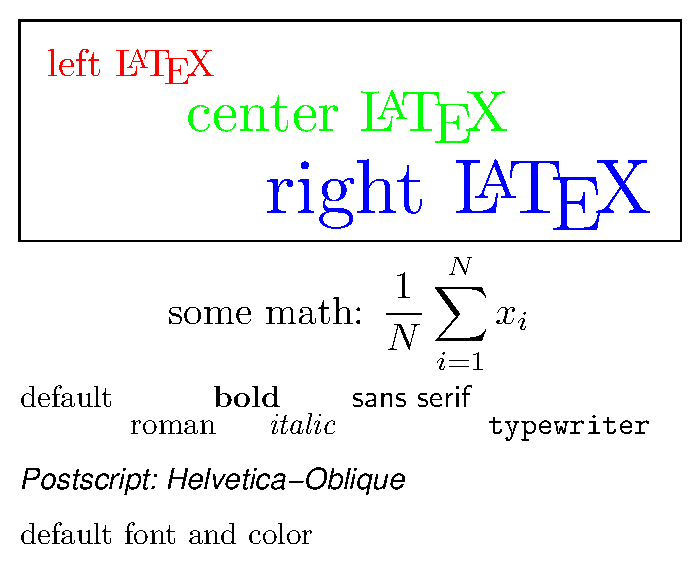
\includegraphics[width=0.5\textwidth]{figuras/test.eps}
	\caption[Esquema do banco de dados do \starlight.]
	{Esquema do banco de dados do \starlight.}
	\label{fig:EsquemaBDStarlight}
\end{figure}

\subsection{Amostra do \starlight}
\label{sec:Crossmatch:AmostraStarlight}

A amostra de galáxias do \starlight contém $926246$ espectros do \SDSS. A
identificação de cada espectro é feita através de um tripleto: a data juliana
média da observação ({\tt MJD}, {\em Mean Julian Date}), a identificação da
placa de suporte das fibras ópticas ({\tt Plate}) e a identificacão da fibra
utilizada para a obtenção do espectro ({\tt FiberID}). Este tripleto ({\tt MJD},
{\tt Plate}, {\tt FiberID}) identifica unicamente um espectro. Porém, é mais
conveniente (e eficiente) ter um identificador único{\footnote{Chave primária
\fixme}} para os registros num banco de dados. No caso do \SDSS, a tabela de
espectros ({\tt SpecObjAll}) tem um identificador chamado {\tt SpecObjID}.
% FIXME: Explicar o que é uma chave primária.

% TODO: Adicionar figura - esquema simplificado da BD do SDSS.
\begin{figure}
	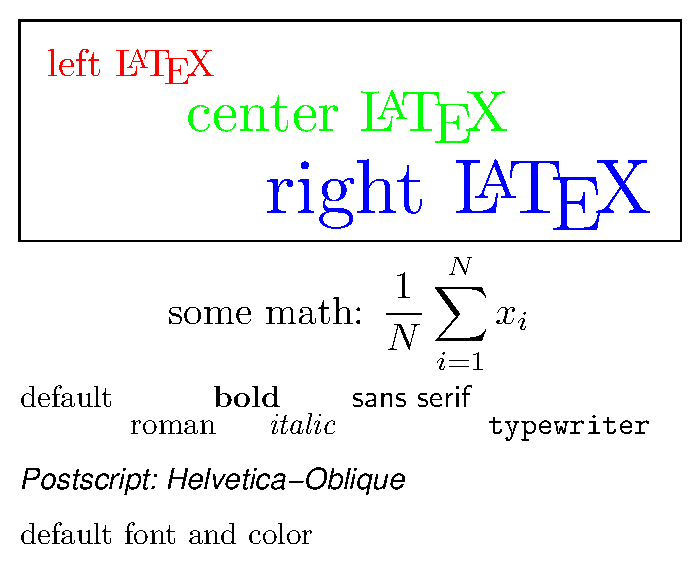
\includegraphics[width=0.5\textwidth]{figuras/test.eps}
	\caption[Esquema do banco de dados do \SDSS.]
	{Esquema do banco de dados do \SDSS.}
	\label{fig:EsquemaSDSS}
\end{figure}

% FIXME: Citação para cobertura do céu do SDSS.
Além de espectros, o banco de dados do \SDSS (figura \ref{fig:EsquemaSDSS})
contém fotometria de $1/4$ do céu.\citneed Os objetos com dados de fotometria
também tem um identificador único, {\tt ObjID}. Existe uma coluna na tabela de
espectros chamada {\tt BestObjID}, que aponta para o registro de fotometria
(tabela {\tt PhotoObjAll}) mais provável para cada espectro. É importante
salientar que nem todo espectro tem um {\tt BestObjID} definido.

A tabela de índices da amostra de galáxias do \starlight (esquema na figura
\ref{fig:TabelaAmostraStarlight}) contém inicialmente os tripletos [{\tt MJD},
{\tt Plate}, {\tt FiberID}]. Dentro do ambiente {CasJobs} do \SDSS
DR7\footnote{{\em CasJobs} \SDSS DR7 - \url{http://casjobs.sdss.org/CasJobs/}} a
tabela tem os valores de {\tt SpecObjID} e {\tt BestObjID} preenchida através da
execução da {\em query} mostrada na figura \ref{fig:AtualizaObjIds}. Entre os
objetos na amostra do \starlight, $622$ objetos não tem a sua contrapartida
fotométrica.

% TODO: Adicionar figura - Tabela amostra do starlight.
\begin{figure}
	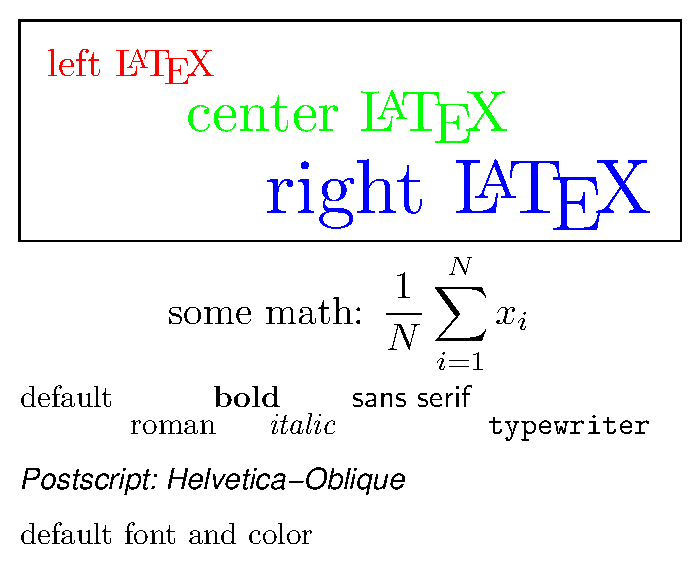
\includegraphics[width=0.5\textwidth]{figuras/test.eps}
	\caption[Esquema da tabela de índices da amostra do \starlight.]
	{Esquema da tabela de índices da amostra do \starlight. Os tipos de dados são
	referentes à implementação do banco de dados.}
	\label{fig:TabelaAmostraStarlight}
\end{figure}

\begin{figure}
	\begin{Verbatim}[commandchars=\\\{\}]
	\textbf{UPDATE} sample
		\textbf{SET} SpecObjID=so.SpecObjID, ObjID=so.BestObjID
	\textbf{FROM} sample s2 \textbf{INNER JOIN} DR7..SpecObjAll so
		\textbf{ON} so.MJD=s2.MJD
		\textbf{AND} so.Plate=s2.Plate
		\textbf{AND} so.FiberID=s2.FiberID
	\end{Verbatim}
	\caption
	[{\em Query} para atualizar os índices da amostra de galáxias do
	\starlight.]
	{Atualização dos índices da amostra de galáxias do \starlight. A {\em query}
	foi executada no {\em CasJobs} do \SDSS DR7 para obter {\tt SpecObjID} e {\tt
	BestObjID} dado o tripleto [{\tt MJD}, {\tt Plate}, {\tt FiberID}].}
	\label{fig:AtualizaObjIds}
\end{figure}


%***************************************************************%
%                                                               %
%                   Crossmatch - SDSS X GALEX                   %
%                                                               %
%***************************************************************%

\section{Crossmatch \SDSS/\galex}
% TODO: Crossmatch SDSS/GALEX.
TODO: Crossmatch SDSS/GALEX. \citet{Budavari2009}.

\subsection{Indexação HTM}
% TODO: Indexação HTM.
TODO: Indexação HTM. \citet{Kunszt2000}.
\begin{verbatim}
The Spatial Indexing used in the Sloan
Digital Sky Survey (SDSS) Science Archive divides the spherical surface into
triangles in a hierarchical scheme resulting in roughly equal surface areas at
each level, which is a big advantage over other schemes. The location of a point
on the sky may be given by the unique index id to any level, refining it with
each step. This naming scheme is being used successfully in other catalogs, too,
like GSC-II and GAIA. The use of the Spatial Index in the SDSS is two-fold, a
level-5 index is used to partition the bulk data, and a high-resolution level-14
index id is assigned to each data point to enable quick lookup and proximity
searches. Use of this indexing scheme in more catalogs will enormously simplify
cross-matching of objects. Using a new computing paradigm, we recently realized
a quantum leap in performance that makes this scheme competitive with
bit-interleaving and requires very little memory. The Flux-space Indexing used
is a traditional k-d tree. The space is 5 dimensional, 5 being the number of
SDSS-filters. The specialization to astronomical data has been achieved by
modeling the location of the main branch in this space and applying the k-d tree
subdivisions only to its confined area. The outliers are indexed separately.
Most of the interesting data points come directly from the outlier part of the
index, with no additional analytical effort. Additionally, the key-lookup index
feature of object-oriented databases is exploited for much-used parameters like
flags.
\end{verbatim}

\subsection{Análise de completeza}
% TODO: Análise de completeza do crossmatch SDSS/GALEX
TODO: Análise de completeza do crossmatch SDSS/GALEX. Tem no paper do
\citet{Budavari2009}, acho que é redundante.


%***************************************************************%
%                                                               %
%      Crossmatch - Definição da amostra Starlight/GALEX        %
%                                                               %
%***************************************************************%

\section{Definição das amostras \SDSS/\starlight e \galex}
\label{sec:Crossmatch:DefAmostras}
% TODO: Definição das amostras a serem usadas no próximo cap. (MGS e LRG).

% TODO: Como foi feito o match.

% TODO: Adicionar figura - tabela xSDSSDR7.
\begin{figure}
	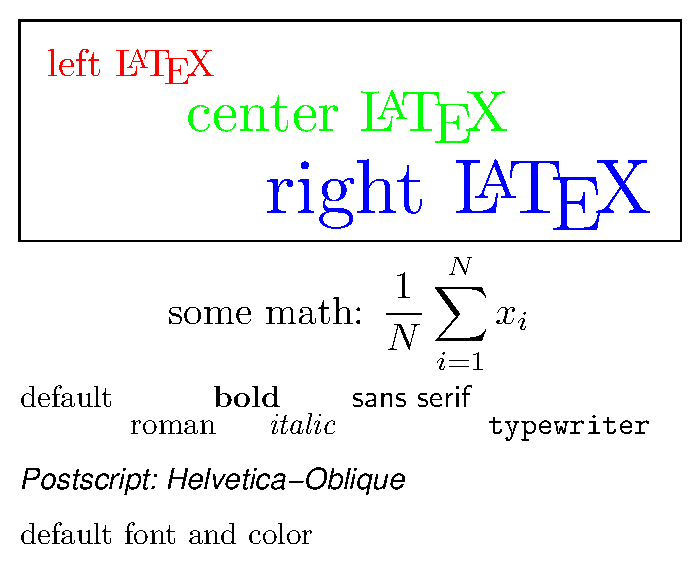
\includegraphics[width=0.5\textwidth]{figuras/test.eps}
	\caption[Esquema da tabela de {em crossmatch} entre objetos do \galex e do
	\SDSS.]
	{Esquema da tabela de {\em crossmatch} entre objetos do \galex e do
	\SDSS.}
	\label{fig:TabelaxSDSSDR7}
\end{figure}

% FIXME: Corrigir caption da figura do match AIS.
\begin{figure}
	\begin{Verbatim}[commandchars=\\\{\}]
	\textbf{SELECT INTO} mydb..galex_ais
		s.objid \textbf{AS} sdssobjid, x.objid \textbf{AS} galexobjid,
		s.mjd, s.plate, s.fiberid,
		g.nuv_mag, nuv_magErr,
		g.fuv_mag, g.fuv_magErr,
		g.e_bv,
		g.band,
		x.distance,
		pe.nexptime,
		pe.fexptime
	\textbf{FROM} mydb..sample s
	\textbf{LEFT JOIN} xSDSSDR7 x
		\textbf{ON} s.objid = x.sdssobjid
		\textbf{AND} x.distanceRank=1
		\textbf{AND} x.reverseDistanceRank=1
		\textbf{AND} x.multipleMatchCount=1
		\textbf{AND} x.reverseMultipleMatchCount=1
	\textbf{LEFT JOIN} photoobjall g
		\textbf{ON} g.objid = x.objid
	\textbf{LEFT JOIN} photoextract e
		\textbf{ON} e.photoextractid=g.photoextractid
	\textbf{WHERE} e.mpstype='AIS'
	\end{Verbatim}
	\caption[{\em Query} para o {\em match} entre os objetos da amostra do
	\starlight e \galex AIS.]
	{{\em Query} para o {\em match} entre os objetos da amostra do \starlight e
	\galex AIS. A mesma {\em query} foi usada para o MIS, trocando apenas o nome da
	tabela para {\tt galex\_mis} e modificando a última linha para {\tt
	e.mpstype='MIS'}.}
	\label{fig:QueryMatchAIS}
\end{figure}


% TODO: Alguma estatística.


\section{Correções na fotometria UV}
\label{sec:Crossmatch:Correcoes}

\subsection{Poeira}
% TODO: Correção por poeira etc.
%a_FUV = 8.29 * ebv
%a_NUV = 8.18 * ebv
%CCM, Schlegel.

\subsection{K-correct}
% TODO: K-correction


%% End of this chapter
